\section{Internet of Things}
\label{sec:IoT}
O termo \textit{Internet of Things} foi usado pela primeira vez pelos fundadores do \textit{MIT Auto-ID Center},
mencionado especialmente pelo britânico Kevin Ashton no ano de 1999, referindo-se especificamente a área de
Gerenciamento da Cadeia de Suprimentos~\cite{kevinashton2009}. Com o passar do tempo, as aplicações utilizando
esse conceito se ampliaram, sendo aplicadas em áreas como transporte, cuidados com a saúde, automação residencial,
entre outras. Devido a essa evolução no paradigma, a definição de \textit{Things} foi se tornando cada vez mais
abrangente, representando desde implantes de monitoramento cardíacos e transponders para identificação animal
até automóveis com sensores integrados, sensores para análise de luminosidade e temperatura.

A \textit{Internet of Things} consiste basicamente em uma rede de objetos físicos (\textit{Things}) que fornecem
informações específicas de seu contexto (\textit{little data}), gerando assim, uma enorme quantidade de dados
desconexos (\textit{big data}) que precisam ser armazenados, processados e apresentados de uma forma eficiente
e de fácil interpretação. O grande valor encontrado no conceito de \textit{Internet of Things} é relação das
informações produzida por essa rede de dispositivos.

\subsection{Aplicações}
Com a facilitação do acesso e integração de uma grande variedade de dispositivos heterogêneos, uma série de
áreas distintas começou a obter vantagens do paradigma, aplicando interpretações dentro de seu contexto
das informações recebidas para criar soluções para seus respectivos problemas.

\label{sec:IoTAp}
\subsubsection{Smart City}
Além das barreiras técnicas, a adoção do paradigma de \textit{Internet of Things} também é prejudicado
pela dificuldade na criação de um modelo de negócio claro e amplamente aceito para atrair investidores
a financiar o desenvolvimento destas tecnologias~\cite{RePEc:zbw:itse13:88475}.
Neste cenário complexo, a aplicação do conceito de \textit{Internet of Things} em um ambiente urbano
pode se tornar particularmente interessante por atender à forte intenção de muitos governos de adotar
soluções TIC (Tecnologias da Informação e Comunicação) para administração pública.

Apesar de não haver uma definição formal amplamente aceita de \textit{Smart City}, a intenção final é de
alcançar uma melhor utilização dos recursos públicos, oferecendo uma melhor qualidade nos serviços oferecidos
aos cidadãos ao mesmo tempo em que reduz os custos operacionais da administração pública~\cite{IoTSmart2014}.
Este objetivo pode ser atingido pela utilização de um \textit{IoT} urbano, como por exemplo uma infraestrutura
para controlar a utilização de iluminação pública baseada no clima ou sensores em latas de lixo para
identificar a melhor rota para seu recolhimento com base em sua utilização. Grandes empresas como a
IBM e a GE tem investido muito nessa área, criando pilotos bem sucedidos de \textit{Smart City}.

\subsubsection{Automação Residencial}
Quando o conceito de uma casa automatizada foi criada 80 anos atrás, muitas limitações técnicas, que perduraram
até pouco tempo, transformaram esse conceito em um sonho inatingível. Com a evolução da internet e a popularização
das tecnologias de conexões sem fio, os dispositivos conectados continuamente à rede em uma casa possibilitaram
trazer essa antiga ideia à realidade. Este conceito, também conhecido como \textit{Smart Home}, está gradualmente
se definindo em relação às tecnologias e aplicações a serem utilizadas~\cite{6418824}.

Atualmente, existem centenas de grandes empresas investindo neste segmento, criando dispositivos e softwares
para otimizar o uso das moradias com soluções para economia de energia elétrica, segurança
através de monitoramento e conforto. Grandes empresas como Samsung e Apple tem feito vastos investimentos
para facilitar a integração de seus dispositivos com o ecossistema de automação residencial criado em cima
do conceito de \textit{Internet of Things}.

\subsubsection{Sistemas Médicos e de Saúde Pessoal}
Uma das áreas de aplicação mais proeminente é a relacionada à saúde. Atualmente existem muitas aplicações
de IoT com o intuito de melhorar a saúde pessoal baseadas em dados como exercícios físicos realizados,
análise da qualidade do sono e alimentação. Grandes empresas como a Apple estão investindo fortemente nessa
área e tornando-a cada vez mais fértil com a criação de novos sensores e interligação de dados.

Ainda dentro da área da saúde, existem aplicações com foco maior na área médica, como, por exemplo,
avaliação de pacientes a distância, possibilitando um atendimento mais rápido e específico baseados em uma
série de informações provenientes de sensores com finalidades distintas como pressão sangüinea,
frequência cardíaca, temperatura, entre outros. Essas aplicações representam um grande avanço, tendo
em vista que pela primeira vez, é possível acessar informações precisas em tempo real, além de possibilitar
a montagem de grupos de teste com uma facilidade sem precedentes. Essa área se tornou tão proeminente que
possui uma terminologia própria, \textit{IoMT} (\textit{Internet of Medical Things}).


\subsection{Sistemas, Plataformas e Ambientes para IoT}
\label{sec:IoTPlataformas}

\subsubsection{Weave}
O Wave é uma linguagem criada pelo Google e anunciada na metade do ano de 2015 que busca um modo padronizado
de possibilitar a comunicação entre dispositivos. Apesar de haver poucas informações devido ao pouco tempo
do anuncio, os exemplos expostos pela empresa propõe um protocolo baseado em uma estrutura JSON e permite a troca
de dados entre SmartPhones Android, a nuvem e outros dispositivos compatíveis.

Possui como foco inicial o conceito de \textit{Smart Home}, entretanto possui grande potencial de
ser utilizado em outros campos, se tornando um sério candidato à protocolo padrão de IoT.

O ponto negativo no presente momento é não possuir muitas informações técnicas ainda, devido ao
curto espaço de tempo que foi divulgado. Espera-se que seja lançado no mercado no final do ano de
2015

\subsubsubsection{Brillo}
Em conjunto com este protocolo, o Google anunciou o lançamento de um sistema operacional desenvolvido em
conjunto com os engenheiros provenientes da empresa Nest, baseado em Android e feito especialmente para
\textit{Internet of Things}, o \textit{Brillo}. O sistema foi desenvolvido com a capacidade de se comunicar
utilizando o protocolo \textit{Weave}, fazendo com que todos os dispositivos utilizando o Brillo se tornem
uma rede de equipamentos conectados, possibilitando o controle e a troca de informação entre estes dispositivos,
a nuvem e dispositivos Android. Com a utilização do protocolo \textit{Weave}, os dispositivos utilizando \textit{Brillo}
serão automaticamente detectados pelos dispositivos Android, semelhante ao funcionamento do protocolo Bonjour~\cite{Bonjour}
mantido pela Apple.

\subsubsection{mbed}
A empresa ARM provê uma solução completa de \textit{Internet of Things} (IoT) chamada mbed\cite{mbed}.
Esta plataforma é dividida em três módulos, mbed OS, mbed Device Server e mbed Tools.\\
A plataforma utiliza em seu sistema embarcado a tecnologia mbedTLS para criptografia de dados com baixo
consumo de memória, desenvolvida inicialmente sob o nome de PolarSSL pela empresa holandesa Offspark,
que foi comprada recentemente pela ARM.

Além de prover uma segurança padrão fim-a-fim entre apps e dispositivos IoT, uma das grandes preocupações
da plataforma mbed é tratar o consumo de energia como uma das principais restrições.

\subsubsubsection{mbed OS}
É um sistema operacional, disponibilizado de graça, para processadores da linha ARM Cortex-M, que são
desenvolvidos visando a eficiência de energia e produtividade.

A arquitetura do mbed OS fornece componentes de software e um framework de aplicação que, combinados
com a grande diversidade de empresas e desenvolvedores que disponibilizam bibliotecas e drivers, facilitam
e agilizam o processo de desenvolvimento de aplicações para IoT.

O mbed OS provê suporte aos padrões como Bluetooth Smart®, Cellular, Thread, Wi-Fi®, e 802.15.4/6LoWPAN junto
com TLS/DTLS, CoAP, HTTP, MQTT e Lightweight M2M

\subsubsubsection{mbed Device Server}
É um produto que possui licença paga e tem como sua funcionalidade principal permitir o gerenciamento
e a conexão dos dispositivos de uma forma segura.

Provê a ligação entre os os protocolos utilizados nos dispositivos IoT e a API que é utilizada por
desenvolvedores web. Isto simplifica a integração de dispositivos IoT que geram \lq little data\rq\ que vão
para os servidores que analisam e agregam a informação gerando a \lq big data\rq.

O Device Server é escalável, podendo conectar e gerenciar milhões de dispositivos.
\begin{figure}[H]
	\centering
		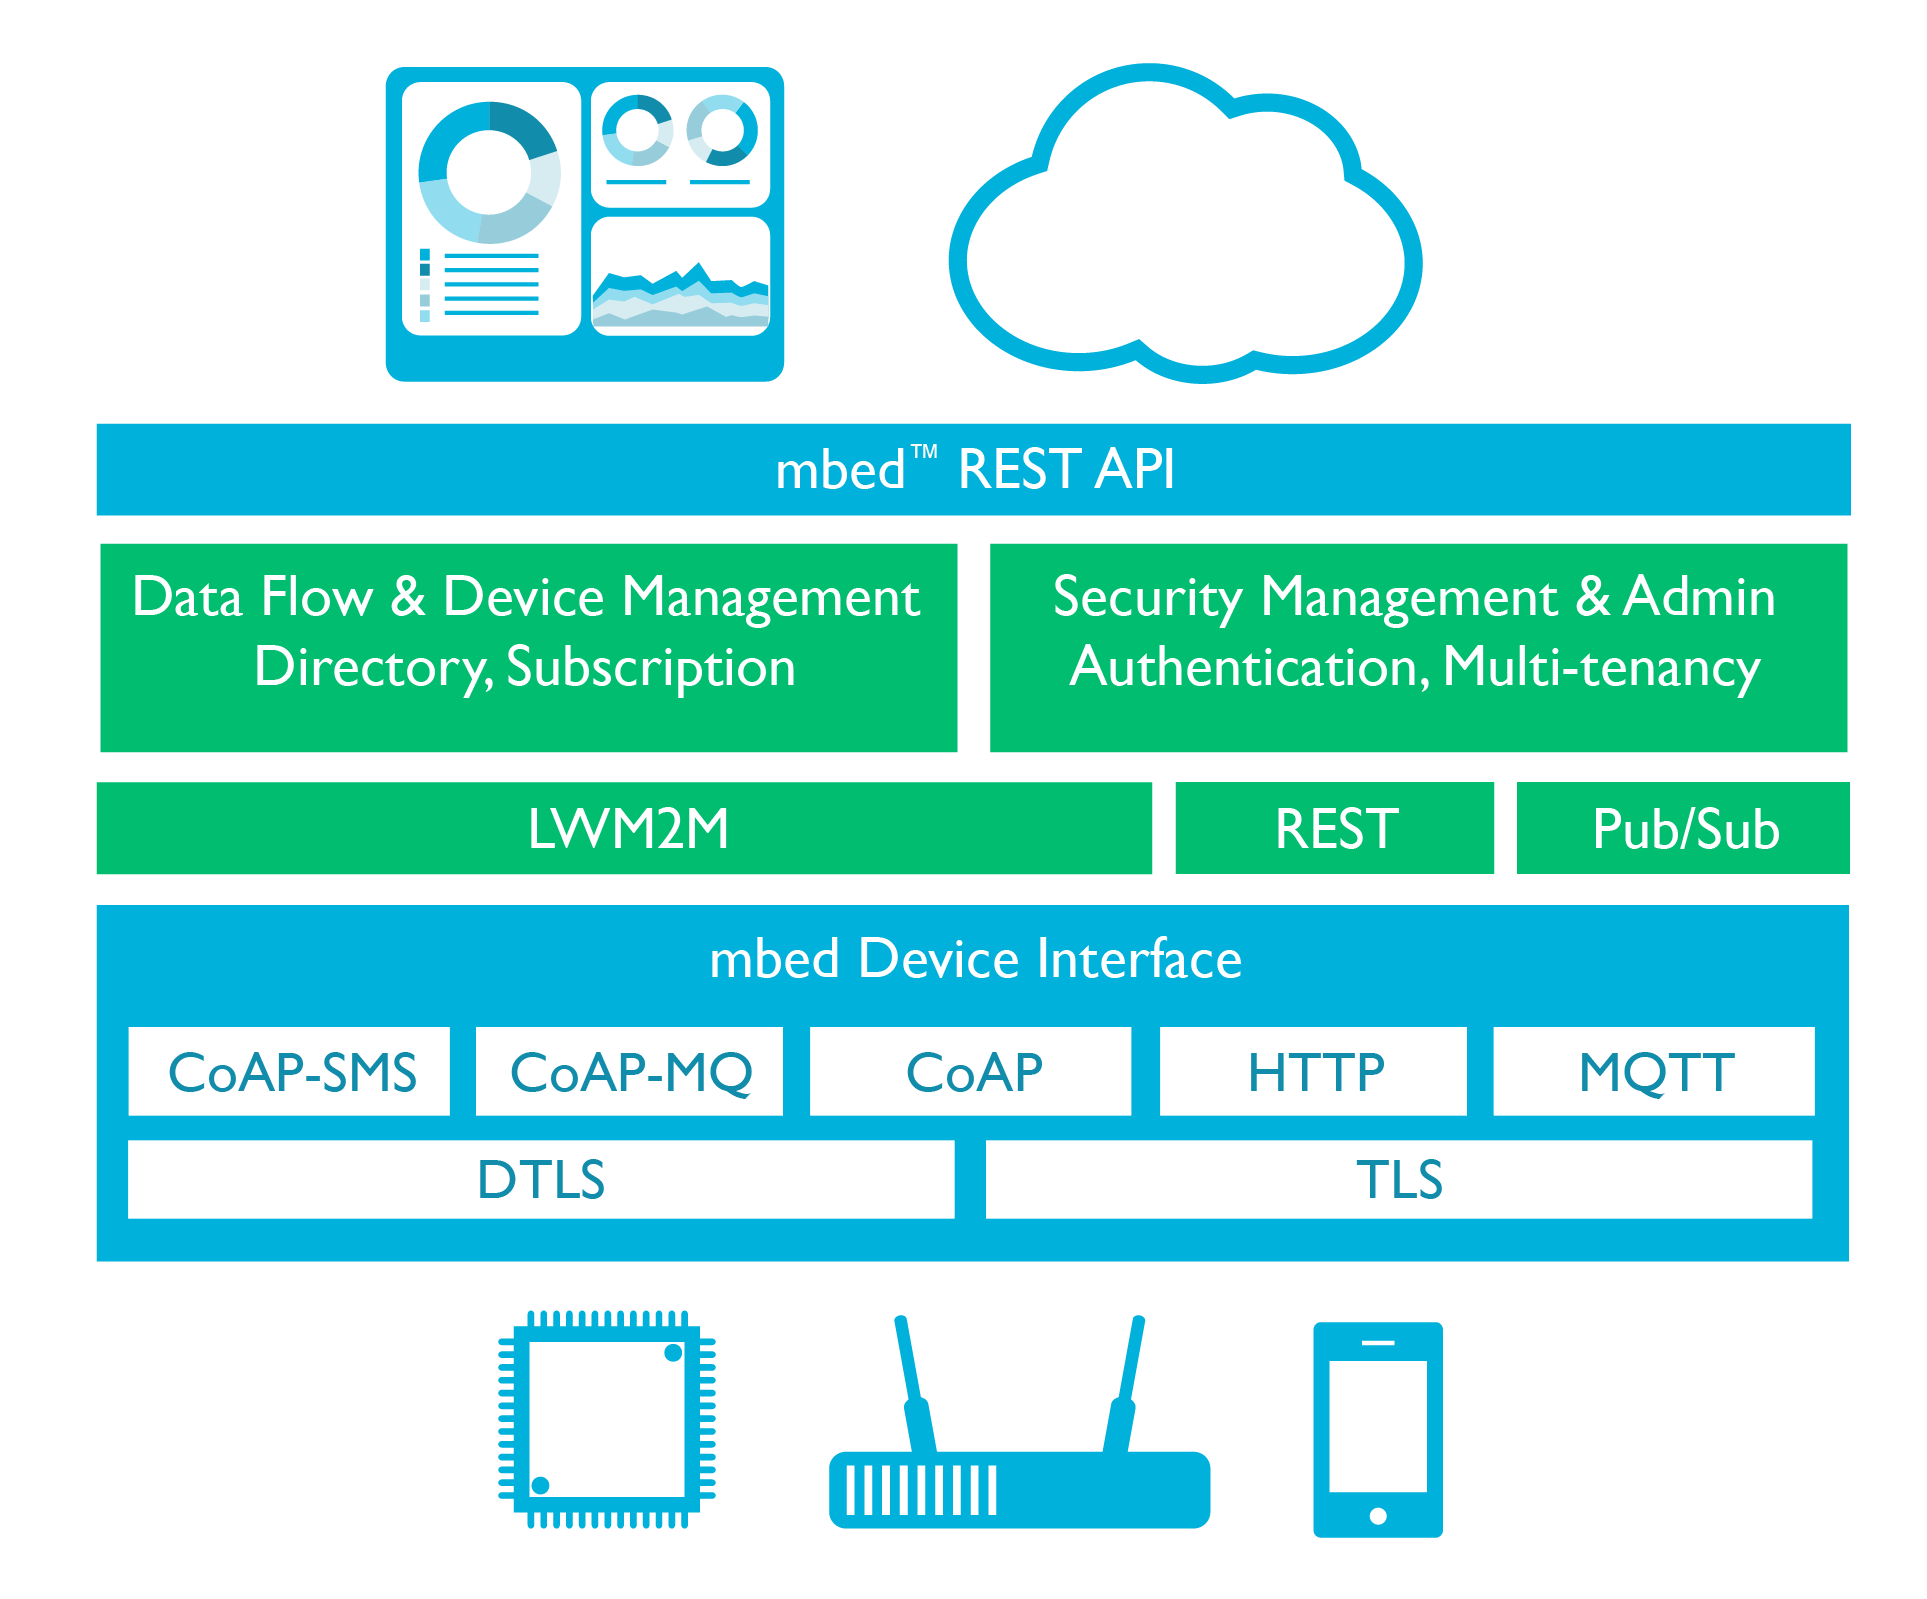
\includegraphics[width=0.7\textwidth]{fig/mbed_arch.png}
	\caption{Arquitetura do mbed Device Server.}
\end{figure}

\subsubsection{FlowCloud}
A tecnologia \textit{FlowCloud} provê uma plataforma segura e independente de aplicações para possibilitar
a rápida construção, gerenciamento e implantação de serviços digitais. Foi desenvolvida pela empresa
Imagination Technologies, que visa com esta solução, suprir as necessidades dos conceitos de
\textit{Internet of Things} e \textit{Machine-to-Machine} (M2M) provendo meios de conectar dispositivos
que estão separados geograficamente, estabelecendo uma conexão ponto a ponto (P2P) entre eles.
A solução visa tratar desde pequenas aplicações de monitoramento em tempo real até grandes serviços
com milhares de usuários~\cite{flowcloud}.

Segundo as especificações descritas pela empresa criadora, as principais funcionalidades do \textit{FlowCloud}
incluem a capacidade de gerenciamento de dispositivos e usuários, serviço de troca de mensagem assíncrona,
registro de eventos, troca de dados de alta segurança e pagamentos eletrônicos. Do ponto de vista analítico,
é fornecida um séria de ferramentas para permitir ao administrador do serviço a criação de relatórios com
utilização de dados em tempo real, capacitando o monitoramento de todas as interações dos usuários e
dispositivos registrados no serviço.

\subsubsection{Arrayent}
Arrayent~\cite{arrayent} é uma plataforma IoT que oferece conexão e segurança entre dispositivos IoT e aplicações
para  smartphones, tablets e web com baixo custo e simplicidade. A plataforma é composta de 4 componentes:
Arrayent Connect Agent, Arreyent Connect Cloud, Arrayent Mobile Framework e Arrayent Cloud Insight.

\subsubsubsection{Arrayent Connect Agent}
É utilizado por desenvolvedores de software embarcado. Funciona como um módulo do firmware que gerencia a
seção do dispositivo com junto ao Arreyent Connect Cloud e abstrai essa responsabilidade para o desenvolvedor
do firmware, deixando-o livre para se preocupar em desenvolver apenas as funcionalidades necessárias para o
funcionamento do dispositivo.

Atualmente a plataforma suporta Wi-Fi, ZigBee, Z-Wave LAN e os sistemas operacionais Linux ou FreeRTOS.

\subsubsubsection{Arrayent Connect Cloud}
O Arrayent Connect Cloud é o coração da plataforma de IoT da Arrayent. Ele é essencialmente um sistema
operacional baseado na cloud que agrega os dispositivos virtualizados, que são uma cópia dos dispositivos
físicos, para que as aplicações web e mobile possam se conectar e recolher informações ou executar comandos
sobre os dispositivos. Além disso, o Arreyent Connect Cloud pode emitir alertas, fazer update de firmware
\lq over-the-air\rq, gerenciar contas de usuários e muito mais.

\subsubsubsection{Arreyent Mobile Framework}
O Arrayent Mobile Framework ajuda os desenvolvedores mobile a criar rapidamente aplicativos intuitivos e
confiáveis para o mercado. Ele abstrai a complexidade envolvida na utilização da plataforma M2M da Arrayent,
que é uma API web de baixo nível, deixando o desenvolvedor livre para se preocupar apenas com as funcionalidades
e beleza dos aplicativos por ele desenvolvidos.

\subsubsubsection{Arrayent Cloud Insight}
O Arrayent Cloud Insight é responsável pela camada de negócio, fornecendo serviços de Business Intelligence,
gerando relatórios de dados comuns a todos os seus produtos como localização do dispositivo, interações entre
os dispositivos e as aplicações, tendência de pico de utilização e muito mais. O Arrayent Cloud Insight agrega,
normaliza, filtra e entrega os dados dos dispositivos para qualquer solução de análise que você utilizar.

\subsubsection{Samsung IoT Plataform}
A plataforma IoT da Samsung provê uma conexão padronizada de diversos dispositivos a um dispositivo
\lq smart\rq\ ou hub.

A Samsung disponibiliza um SDK que simplifica o desenvolvimento de novos serviços, coletando
e processando os dados de sensores e serviços que o usuário possa ter. Os desenvolvedores não precisam analisar ou
fazer setup da infraestrutura complexa de conexão entre os dispositivos ou se preocupar com os dados do usuário na cloud.

A plataforma de IoT da Samsung foi desenhada para que os desenvolvedores se concentrem apenas nas funcionalidades
dos serviços que estão sendo desenvolvidos por eles. Uma limitação do SDK da Samsung é que ele é disponibilizado
apenas para a plataforma Android 4.1 ou superior.

\subsubsection{IBM Internet of Things Foundation}
A IBM desenvolveu a \textit{IBM Internet of Things Foundation}, que consiste em um sistema na nuvem que torna simples
extrair valor dos dispositivos \textit{Internet of Things}. Combinada com a plataforma IBM Bluemix\texttrademark,
é possível acessar dispositivos e dados rapidamente, bem como compor aplicações de análise, aplicativos móveis 
e até um painel de visualizações.

A \textit{IBM Internet of Things Foundation} provê amplo suporte aos seus usuários
disponibilizando diversos manuais e tutoriais que explicam desde o que é a \textit{Internet of Things}
até a documentação detalhada das APIs.

\subsubsubsection{IBM Bluemix}
O \textit{IBM Bluemix} é uma solução de nuvem da IBM que permite aos desenvolvedores a criação
e gerenciamento de aplicativos na nuvem de uma maneira ágil e fácil.
O BlueMix é uma implementação da Arquitetura de Nuvem Aberta da IBM baseada em Cloud Foundry, uma plataforma como serviço (PaaS) de código aberto.

\subsubsection{SmartSantander}
O \textit{SmartSantander} propõe uma instalação de pesquisa única no mundo, em uma escala de uma cidade,
para fomentar o desenvolvimento de serviços e aplicações para uma \textit{Smart City}.
Os resultados de pesquisas efetuadas nesse ambiente devem influenciar as definições e especificações da arquitetura da
Internet do Futuro do ponto de vista dos serviços de \textit{Internet of Things}~\cite{citeulike:13508566}.

O SmartSantander irá possuir mais de 20.000 sensores para IoT em um cenário urbano. O projeto pretende promover os
seguintes resultados~\cite{smartsantandersite}.
\begin{enumerate}
\item Validação das abordagens de modelos arquiteturais da \textit{Internet of Things}.
\item Identificação dos pontos chave para criação de IoT, particularmente os protocolos e mecanismos de gerenciamento e
interação; tecnologia de dispositivos e serviços como localização, identificação, gerenciameno e segurança.
\item Identificação da aceitação das tecnologias e serviços de IoT.
\end{enumerate}

\begin{figure}[H]
	\centering
		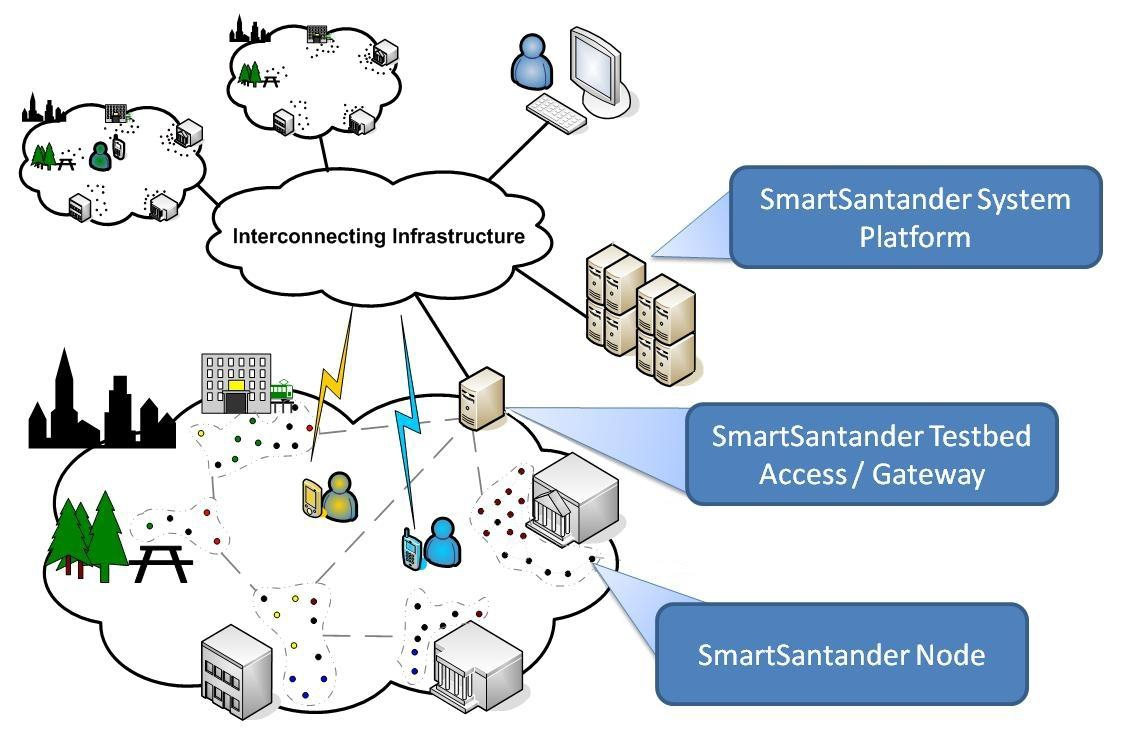
\includegraphics[width=0.7\textwidth]{fig/smartsantander.jpg}
	\caption{Funcionamento da infraestrutura do projeto SmartSantander em alto nível.}
\end{figure}

As instalações experimentais propostas pelo \textit{SmartSantander} precisam atender uma série de demandas
de diferentes \textit{stakeholders}, desde desenvolvedores de soluções e provedores de serviços IoT até os usuários finais.
Vários requisitos funcionais e não-funcionais foram levantados no princípio do projeto, levando em consideração
os variados pontos de vista e necessidades dos \textit{stakeholders} envolvidos. Os resultados foram divididos em quatro
aspectos, criando o modelo arquitetura com os subsistemas descritos a seguir~\cite{citeulike:13508566}:


\subsubsubsection{Authentication, Authorisation and Accounting (AAA)}
Implementa funções que controlam e auditam o acesso à todas as funcionalidades do sistema. Possui processos
comuns entre todos os tipos de usuários da instalação. Representa tipicamente o primeiro ponto de contato
do usuário para que esse tenha acesso às demais funcionalidades do ambiente de testes, o \textit{Testbed}.
Além das funcionalidades de gerenciamento das contas de usuários no ambiente de teste, as funções
do AAA garante que o usuário está propriamente autenticado e que possui a autorização necessária para
acessar o ambiente de teste de acordo com suas permissões.

\subsubsubsection{Testbed Management}
O \textit{Testbed Management} engloba as funções que são relevantes para a operação do ambiente de teste.
Este subsistema provê uma série de funcionalidades, como por exemplo configuração \textit{plug and play}
de novos componentes do \textit{testbed}, monitoramento e avaliação de performance.

\subsubsubsection{Experimental Support}

O \textit{Experimental Support} provê todas as funcionalidades relativas ao ciclo de vida dos usuários
do ambiente de teste. As funcionalidades são geralmente utilizadas por pesquisadores, mas também são utilizadas por
provedores de sistemas, já que um sistema pode ser visto como um experimento de longa duração.
Suas funcionalidades incluem funções para verificar a ocupação dos recursos no ambiente de testes e suas características,
mecanismos para configurar os experimentos, controle dos experimentos e análise de dados.

\subsubsubsection{Application Support}
O \textit{Application Support} provê funcionalidades para serem utilizadas por desenvolvedores de aplicações
e provedores de serviços para compor um \textit{Smart Service} rodando nas instalações do \textit{SmartSantander}.
Estas são ferramentas para acessar facilmente informações de sensores e gerenciar dados.

\subsubsection{FIWARE}
O FIWARE é uma iniciativa para promover um ecossistema que capture as oportunidades que surgirão com a nova onda
de digitalização causada pela integração das novas tecnologias relacionadas à Internet. Esse projeto é
baseado nos cinco módulos descritos a seguir.

\subsubsubsection{FIWARE}
A plataforma FIWARE provê um simples porém poderoso conjunto de APIs que facilitam o desenvolvimento de \textit{Smart Applications}
em uma séries de setores. As APIs disponibilizadas possuem uma especificação pública e sem necessidade de pagamento de royalties.
Além das APIs, cada componente do FIWARE possui uma implementação como referência com código de fonte aberto e distribuída
publicamente, possibilitando que mais provedores de solução entrem no mercado de maneira rápida e com baixo custo.

\subsubsubsection{FIWARE Lab}
Experimentos realizados em ambiente real aceleram o desenvolvimento das tecnologias da Internet do Futuro e seus serviços,
qualificam o mercado de infraestruturas \textit{Smart}, para possibilitar isso, o \textit{FIWARE Lab} foi criado.
O \textit{FIWARE Lab} é um ambiente de teste não comercial criado para que a experimentação e inovação baseada nas tecnologias
FIWARE sejam fomentadas. Investidores, desenvolvedores e demais interessados podem testar a tecnologia e suas aplicações neste
ambiente, se utilizando de \textit{Open Data} publicada por cidades e organizações. O \textit{FIWARE Lab} é aplicado sobre
uma rede geograficamente distribuída de nodos interligados criando uma grande infraestrutura experimental~\cite{7027596}.

\subsubsubsection{FIWARE Ops}
O \textit{FIWARE Ops} é uma coleção de ferramentas para facilitar a implantação, configuração e operação das instâncias de FIWARE.
Este conjunto de ferramentas foi desenvolvido para ajudar na expansão da infraestrutura associada a uma instância de FIWARE
adicionando novos nodos com o passar do tempo e permitindo a cooperação de múltiplos provedores de plataformas. Em resumo,
o \textit{FIWARE Ops} é a ferramente utilizada para montar, operar e expandir o \textit{FIWARE Lab}.

\subsubsubsection{FIWARE Accelerate}
O \textit{FIWARE Acceleration Programme} busca promover a adoção das tecnologias FIWARE por parte dos integradores de
soluções e desenvolvedores de aplicações com foco especial nos especialistas e start-ups. A União Europeia iniciou uma
campanha ambiciosa em setembro de 2014, financiando com 80 milhões de euros especialistas e empreendedores que tenham
intenção de desenvolver aplicações inovadoras baseadas na tecnologia FIWARE.

\subsubsubsection{FIWARE Mundus}
Mesmo tendo surgido na Europa, o FIWARE foi desenvolvido com uma ambição de adoção global. O \textit{FIWARE Mundus} é um programa
criado para para atingir esse objetivo, envolvendo investidores e interessados de outras regiões do mundo para participarem
no desenvolvimento e utilização das tecnologias.
